\documentclass[tikz,border=10pt]{standalone}
% No extra TikZ libraries needed
\begin{document}
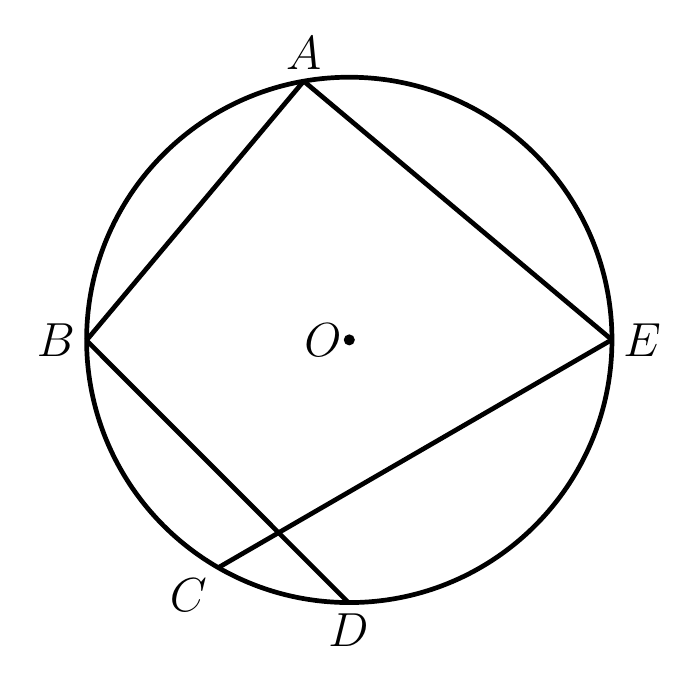
\begin{tikzpicture}[line join=round, line width=1.7pt]
  % Scale s = 0.02122 cm/px (from STYLE METRICS), origin at O (px 225.98, 220.25)
  \coordinate (O) at (0,0);
  \coordinate (A) at (-0.579,3.286);   % top
  \coordinate (B) at (-3.338,-0.006);  % left
  \coordinate (E) at (3.334,0.002);    % right
  \coordinate (C) at (-1.663,-2.892);  % bottom-left
  \coordinate (D) at (-0.011,-3.336);  % bottom

  % Circle centred at O, radius 157.2 px = 3.336 cm
  \draw (O) circle (3.336);

  % Chords
  \draw (A) -- (B);
  \draw (A) -- (E);
  \draw (B) -- (D);
  \draw (E) -- (C);

  % Centre dot: filled, radius about 2pt
  \fill (O) circle (2pt);

  % Labels
  \node[above, font=\fontsize{17}{20.4}\selectfont] at (A) {$A$};
  \node[left, font=\fontsize{17}{20.4}\selectfont] at (B) {$B$};
  \node[right, font=\fontsize{17}{20.4}\selectfont] at (E) {$E$};
  \node[below left, font=\fontsize{17}{20.4}\selectfont] at (C) {$C$};
  \node[below, font=\fontsize{17}{20.4}\selectfont] at (D) {$D$};
  % O label moved to the left of the centre dot
  \node[left, font=\fontsize{17}{20.4}\selectfont, inner sep=2pt] at (O) {$O$};
\end{tikzpicture}
\end{document}